\documentclass[11pt]{article}
\usepackage{listings}
\usepackage{graphicx}
\usepackage[parfill]{parskip}

%Gummi|065|=)
\title{\textbf{COP5615 - Distributed Operating Systems\\Project 3: Chord}}
\author{Rahul Prabhu\\
		Sanil Sinai Borkar}
\date{\today}
\begin{document}

\maketitle
\section{Description}

We used sbt to run our program. The following command was run at the sbt command prompt:
\begin{lstlisting}
$ run <numNodes> <numRequests>
\end{lstlisting}


There are 2 command-line arguments as given below:
\begin{enumerate}
\item \textbf{numNodes}: The number of nodes in the Chord P2P network. It is a positive integer value.
\item \textbf{numRequests}: The number of requests that each peer node has to make. One such request will be made per second.
\end{enumerate}

sbt will prompt to select the main class. Please select\\ {\it edu.zeroday.chord.Chord}

Once all the nodes make {\it numRequests} message requests, the program exits.

\section{Chord}
Chord works on the principle of keeping track of its neighbors in its finger tables, which are located at distances of powers of 2 from itself. When searching for a query it makes use of its finger tables to find the closest preceding node to the query being searched, and this node will then do the same.

We have selected m = 20. Therefore, the maximum network size is $2^m = 1048576$, with node IDs lying in the range $[0, 1048576)$.

We ran the Chord on varying network sizes. Figure~\ref{chordresults} shows the results of the average number of hops taken to deliver a fixed number of messages (100 messages per node) for varying network sizes. 

\textit{The algorithm was run several times for each test instance, and the times shown are averages over these runs.}

\begin{figure}[h]
    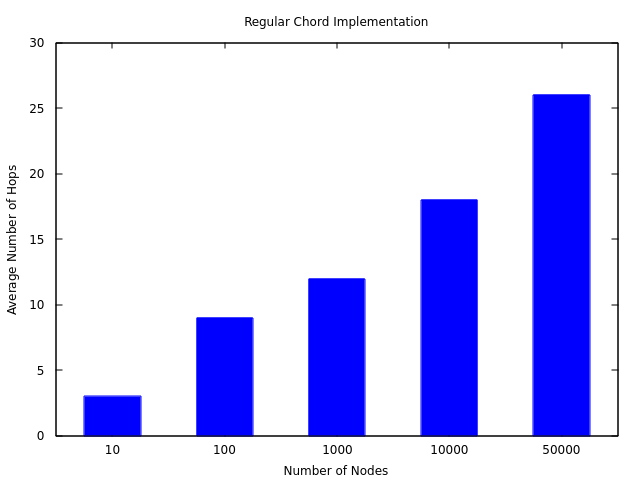
\includegraphics[scale=0.75]{images/regularchord.png}
    \caption{Chord run on various network sizes}
    \label{chordresults}
\end{figure}


\section{Observations}
Since we are not making use of concurrent node joins, the nodes join the network synchronously. Moreover, once a new node joins, it may need to update the finger tables of its predecessors. Since this update is done synchronously, the network takes time to build up before we can start querying.

As the Chord paper says, the program requires $O$(log N) hops to deliver a message in a network of N nodes (peers). This is only possible if the finger tables of every node are up to date, which may not always be the case. As the paper suggests, there are 3 possibilities which can occur during lookup:
\begin{enumerate}
\item The finger tables, successors, and predecessors are up to date - the algorithm runs correctly and lookup takes O(log N) time
\item The finger tables are stale, but successors and predecessors are up to date - the algorithm runs correctly but lookup takes longer than O(log N) time which may be O(N) time in the worst case.
\item The finger tables, successors, and predecessors are stale - the algorithm fails and lookup may not be possible. This is analyzed in our failure (bonus) part.
\end{enumerate}

As the Chord paper suggests, if the number of hops encountered were too huge, Chord does not use the closest preceding finger entry to forward the request but rather send the message to its successor, which in turn sends it to its successor, and so on, eventually hoping that the node responsible for the message will be encountered. However, this process takes a longer time which could potentially be O(N). In our case, Chord took a lot of time but lookup was done successfully due to this alternative lookup scheme.

To verify that the message was delivered to the required node, we had stored a message at each node in the form of ``Message" followed by the node ID. For example, Node 123 will store the message \textit{Message123}. So if a node was looking up a query for which is some node {\it X} was responsible, then that node {\it X} will reply to the request initiator with \textit{MessageX}. In the process of such lookup, the average number of hops were calculated, which were then eventually printed on the screen.

{\it Note: The query to lookup is generated randomly for each node. Therefore, it depends on the random number generator in Scala how actually random these IDs to be queried are, to achieve a ``truly" random query lookup.}

\end{document}
